% figures/new/fig_wtpnet.tex -- Figure 4 (fig:wtpnet), written by W2b. Self-contained float (BLUEPRINT 2.10 exhibit; Override O6).
% Input from sections/10_menu.tex. Scatter of WTP (vertical) against Net (horizontal), one marker per row of the five
% May 2025 reform tables; marker type by family. Built only from printed cells; no number is computed here.
% Coordinates are written (Net, WTP). Cells were extracted from the table files by scratchpad/w2b_tools/make_fig.py
% and checked against dossier 03 section 4.2-4.7 and BLUEPRINT 8.8-8.10 on 2026-11-09.
% Cells (WTP, Net) by row -- file:line in tables/:
%   AN1         WTP  -0.38  Net  -0.87   welfare_age_dependence_mvpfv5.tex:108
%   AN2         WTP  -0.74  Net  -1.75   welfare_age_dependence_mvpfv5.tex:109
%   AN3         WTP  -1.09  Net  -2.38   welfare_age_dependence_mvpfv5.tex:110
%   AD1         WTP   0.16  Net  -0.45   welfare_age_dependence_mvpfv5.tex:112
%   AD2         WTP   0.19  Net  -0.44   welfare_age_dependence_mvpfv5.tex:113
%   AD3         WTP   0.23  Net  -0.66   welfare_age_dependence_mvpfv5.tex:114
%   AD4         WTP   0.26  Net  -0.73   welfare_age_dependence_mvpfv5.tex:115
%   AD5         WTP    0.3  Net  -0.78   welfare_age_dependence_mvpfv5.tex:116
%   AL1         WTP   0.10  Net  -0.12   welfare_age_dependence_mvpfv5.tex:118
%   AL2         WTP   0.15  Net  -0.46   welfare_age_dependence_mvpfv5.tex:119
%   AL3         WTP   0.21  Net  -0.72   welfare_age_dependence_mvpfv5.tex:120
%   AL4         WTP   0.29  Net  -0.86   welfare_age_dependence_mvpfv5.tex:121
%   AL5         WTP   0.37  Net  -1.17   welfare_age_dependence_mvpfv5.tex:122
%   AL6         WTP   0.47  Net  -1.37   welfare_age_dependence_mvpfv5.tex:123
%   AL7         WTP   0.57  Net  -1.38   welfare_age_dependence_mvpfv5.tex:124
%   AL8         WTP   0.69  Net  -1.47   welfare_age_dependence_mvpfv5.tex:125
%   AL9         WTP   0.80  Net  -1.57   welfare_age_dependence_mvpfv5.tex:126
%   P1.1        WTP   0.10  Net  -0.03   welfare_progressivity_mvpfv7.tex:115
%   P1.2        WTP   0.22  Net   0.09   welfare_progressivity_mvpfv7.tex:116
%   P1.3        WTP   0.31  Net   0.13   welfare_progressivity_mvpfv7.tex:117
%   P1.4        WTP   0.40  Net   0.19   welfare_progressivity_mvpfv7.tex:118
%   P1.5        WTP   0.50  Net   0.21   welfare_progressivity_mvpfv7.tex:119
%   P1.6        WTP   0.59  Net   0.20   welfare_progressivity_mvpfv7.tex:120
%   P1.7        WTP   0.67  Net   0.26   welfare_progressivity_mvpfv7.tex:121
%   P1.8        WTP   0.75  Net   0.34   welfare_progressivity_mvpfv7.tex:122
%   P1.9        WTP   0.80  Net   0.44   welfare_progressivity_mvpfv7.tex:123
%   P2.0        WTP   0.83  Net   0.57   welfare_progressivity_mvpfv7.tex:126
%   P2.1        WTP   0.86  Net   0.67   welfare_progressivity_mvpfv7.tex:127
%   P2.2        WTP   0.88  Net   0.70   welfare_progressivity_mvpfv7.tex:128
%   P2.3        WTP   0.90  Net   0.78   welfare_progressivity_mvpfv7.tex:129
%   P2.4        WTP   0.92  Net   0.93   welfare_progressivity_mvpfv7.tex:130
%   P2.5        WTP   0.93  Net   0.98   welfare_progressivity_mvpfv7.tex:131
%   P2.6        WTP   0.95  Net   1.03   welfare_progressivity_mvpfv7.tex:132
%   P2.7        WTP   0.94  Net   1.11   welfare_progressivity_mvpfv7.tex:133
%   P2.8        WTP   0.95  Net   1.19   welfare_progressivity_mvpfv7.tex:134
%   P2.9        WTP   0.95  Net   1.27   welfare_progressivity_mvpfv7.tex:135
%   P3.0        WTP   0.95  Net   1.26   welfare_progressivity_mvpfv7.tex:137
%   P3.1        WTP   0.96  Net   1.27   welfare_progressivity_mvpfv7.tex:138
%   P3.2        WTP   0.96  Net   1.28   welfare_progressivity_mvpfv7.tex:139
%   P3.3        WTP   0.96  Net   1.26   welfare_progressivity_mvpfv7.tex:140
%   P3.4        WTP   0.96  Net   1.27   welfare_progressivity_mvpfv7.tex:141
%   P3.5        WTP   0.97  Net   1.29   welfare_progressivity_mvpfv7.tex:142
%   P3.6        WTP   0.97  Net   1.27   welfare_progressivity_mvpfv7.tex:143
%   P3.7        WTP   0.97  Net   1.27   welfare_progressivity_mvpfv7.tex:144
%   P3.8        WTP   0.97  Net   1.25   welfare_progressivity_mvpfv7.tex:145
%   P3.9        WTP   0.98  Net   1.24   welfare_progressivity_mvpfv7.tex:146
%   L0          WTP   0.16  Net   0.12   welfare_progressivity_mvpfv7.tex:149
%   L1          WTP   0.32  Net   0.21   welfare_progressivity_mvpfv7.tex:150
%   L2          WTP   0.46  Net   0.36   welfare_progressivity_mvpfv7.tex:151
%   L3          WTP   0.60  Net   0.38   welfare_progressivity_mvpfv7.tex:152
%   L4          WTP   0.74  Net   0.49   welfare_progressivity_mvpfv7.tex:153
%   L5          WTP   0.87  Net   0.64   welfare_progressivity_mvpfv7.tex:154
%   L6          WTP   0.95  Net   0.79   welfare_progressivity_mvpfv7.tex:155
%   L7          WTP   1.00  Net   0.92   welfare_progressivity_mvpfv7.tex:156
%   L8          WTP   1.02  Net   1.14   welfare_progressivity_mvpfv7.tex:157
%   L9          WTP   0.98  Net   1.24   welfare_progressivity_mvpfv7.tex:158
%   Medicare A  WTP   1.36  Net   3.53   welfare_medicare_mvpfv8.tex:113
%   Medicare B  WTP   1.30  Net   3.19   welfare_medicare_mvpfv8.tex:116-118
%   I1          WTP   0.44  Net   0.69   welfare_tax_mvpf_v8.tex:114
%   I2          WTP   0.87  Net   1.28   welfare_tax_mvpf_v8.tex:115
%   I3          WTP   1.29  Net   2.01   welfare_tax_mvpf_v8.tex:116
%   I4          WTP   1.69  Net   2.80   welfare_tax_mvpf_v8.tex:117
%   I5          WTP   2.09  Net   3.46   welfare_tax_mvpf_v8.tex:118
%   K1          WTP   0.87  Net   0.08   welfare_savings_mvpf_v3.tex:120
%   K2          WTP   1.75  Net   0.18   welfare_savings_mvpf_v3.tex:122
%   K3          WTP    3.6  Net   1.34   welfare_savings_mvpf_v3.tex:123
% Note: L9 and P3.9 are the same policy and plot at the same point (0.98, 1.24); AD1 (-0.45, 0.16) and AL2 (-0.46, 0.15) nearly coincide.
% House style: grid, legend below the axis, FROT palette from preamble.tex (blue, red, green) plus black.
\begin{figure}[!t]
\centering
\caption{Willingness to Pay and Net Fiscal Effect across Reform Families}
\label{fig:wtpnet}
\vspace{6pt}
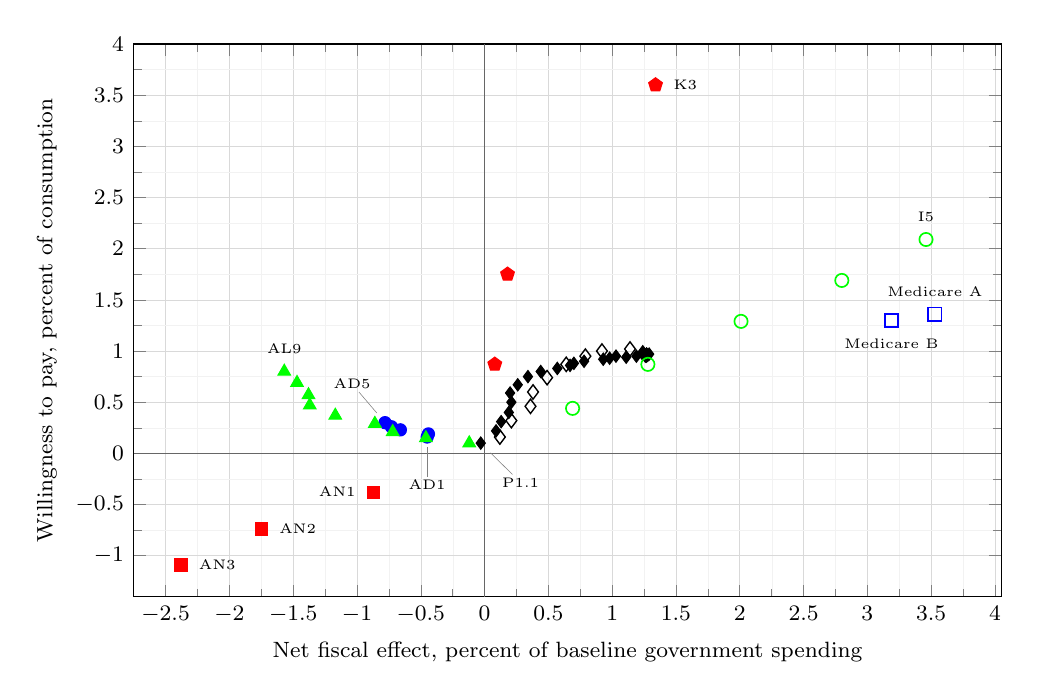
\begin{tikzpicture}
\begin{axis}[%
width=12.6cm,
height=8.6cm,
xlabel={Net fiscal effect, percent of baseline government spending},
ylabel={Willingness to pay, percent of consumption},
xmin=-2.75, xmax=4.05,
ymin=-1.4, ymax=4.0,
xtick={-2.5,-2,...,4},
ytick={-1,-0.5,...,4},
grid=both,
grid style={line width=0.2pt, draw=gray!30},
minor grid style={line width=0.1pt, draw=gray!10},
minor tick num=1,
axis background/.style={fill=white},
tick label style={font=\footnotesize},
label style={font=\footnotesize},
legend to name=legwtpnet,
legend columns=4,
legend style={draw=white!15!black, font=\scriptsize, /tikz/every even column/.append style={column sep=0.6em}},
legend cell align=left,
clip=false
]
% zero lines
\addplot [forget plot, black!60, line width=0.4pt] coordinates {(-2.75,0) (4.05,0)};
\addplot [forget plot, black!60, line width=0.4pt] coordinates {(0,-1.4) (0,4.0)};
% AN1-AN3                                                          % src: tables/welfare_age_dependence_mvpfv5.tex:108-110
\addplot [only marks, color=red, mark=square*, mark size=2.2pt] coordinates {(-0.87,-0.38) (-1.75,-0.74) (-2.38,-1.09)};
\addlegendentry{Higher NRA (AN1--AN3)}
% AD1-AD5                                                          % src: tables/welfare_age_dependence_mvpfv5.tex:112-116
\addplot [only marks, color=blue, mark=*, mark size=2.2pt] coordinates {(-0.45,0.16) (-0.44,0.19) (-0.66,0.23) (-0.73,0.26) (-0.78,0.3)};
\addlegendentry{Higher DRC (AD1--AD5)}
% AL1-AL9                                                          % src: tables/welfare_age_dependence_mvpfv5.tex:118-126
\addplot [only marks, color=green, mark=triangle*, mark size=2.6pt] coordinates {(-0.12,0.10) (-0.46,0.15) (-0.72,0.21) (-0.86,0.29) (-1.17,0.37) (-1.37,0.47) (-1.38,0.57) (-1.47,0.69) (-1.57,0.80)};
\addlegendentry{Symmetric adjustment (AL1--AL9)}
% P1.1-P1.9, P2.0-P2.9, P3.0-P3.9                                  % src: tables/welfare_progressivity_mvpfv7.tex:115-123, 126-135, 137-146
\addplot [only marks, color=black, mark=diamond*, mark size=2.2pt] coordinates {(-0.03,0.10) (0.09,0.22) (0.13,0.31) (0.19,0.40) (0.21,0.50) (0.20,0.59) (0.26,0.67) (0.34,0.75) (0.44,0.80) (0.57,0.83) (0.67,0.86) (0.70,0.88) (0.78,0.90) (0.93,0.92) (0.98,0.93) (1.03,0.95) (1.11,0.94) (1.19,0.95) (1.27,0.95) (1.26,0.95) (1.27,0.96) (1.28,0.96) (1.26,0.96) (1.27,0.96) (1.29,0.97) (1.27,0.97) (1.27,0.97) (1.25,0.97) (1.24,0.98)};
\addlegendentry{Progressivity (P1.1--P3.9)}
% L0-L9                                                            % src: tables/welfare_progressivity_mvpfv7.tex:149-158
\addplot [only marks, color=black, mark=diamond, mark size=2.6pt, line width=0.5pt] coordinates {(0.12,0.16) (0.21,0.32) (0.36,0.46) (0.38,0.60) (0.49,0.74) (0.64,0.87) (0.79,0.95) (0.92,1.00) (1.14,1.02) (1.24,0.98)};
\addlegendentry{Level (L0--L9)}
% Medicare Part A, Part B                                          % src: tables/welfare_medicare_mvpfv8.tex:113, 116-118
\addplot [only marks, color=blue, mark=square, mark size=2.4pt, line width=0.6pt] coordinates {(3.53,1.36) (3.19,1.30)};
\addlegendentry{Medicare Part A, Part B}
% I1-I5                                                            % src: tables/welfare_tax_mvpf_v8.tex:114-118
\addplot [only marks, color=green, mark=o, mark size=2.4pt, line width=0.6pt] coordinates {(0.69,0.44) (1.28,0.87) (2.01,1.29) (2.80,1.69) (3.46,2.09)};
\addlegendentry{Income tax (I1--I5)}
% K1-K3                                                            % src: tables/welfare_savings_mvpf_v3.tex:120, 122, 123
\addplot [only marks, color=red, mark=pentagon*, mark size=2.6pt] coordinates {(0.08,0.87) (0.18,1.75) (1.34,3.6)};
\addlegendentry{Saving subsidy (K1--K3)}
% point labels (selected rows)
\node [anchor=east, font=\tiny, xshift=-3pt] at (axis cs:-0.87,-0.38) {AN1};     % src: tables/welfare_age_dependence_mvpfv5.tex:108
\node [anchor=west, font=\tiny, xshift=3pt] at (axis cs:-1.75,-0.74) {AN2};     % src: tables/welfare_age_dependence_mvpfv5.tex:109
\node [anchor=west, font=\tiny, xshift=3pt] at (axis cs:-2.38,-1.09) {AN3};     % src: tables/welfare_age_dependence_mvpfv5.tex:110
\node [pin={[pin distance=11pt, font=\tiny, inner sep=1pt]270:AD1}] at (axis cs:-0.45,0.16) {};   % src: tables/welfare_age_dependence_mvpfv5.tex:112
\node [pin={[pin distance=8pt, font=\tiny, inner sep=1pt]110:AD5}] at (axis cs:-0.78,0.3) {};    % src: tables/welfare_age_dependence_mvpfv5.tex:116
\node [anchor=south, font=\tiny, yshift=3pt] at (axis cs:-1.57,0.80) {AL9};     % src: tables/welfare_age_dependence_mvpfv5.tex:126
\node [pin={[pin distance=9pt, font=\tiny, inner sep=1pt]300:P1.1}] at (axis cs:-0.03,0.10) {};  % src: tables/welfare_progressivity_mvpfv7.tex:115
\node [anchor=south, font=\tiny, yshift=3pt] at (axis cs:3.53,1.36) {Medicare A}; % src: tables/welfare_medicare_mvpfv8.tex:113
\node [anchor=north, font=\tiny, yshift=-3pt] at (axis cs:3.19,1.30) {Medicare B}; % src: tables/welfare_medicare_mvpfv8.tex:116-118
\node [anchor=south, font=\tiny, yshift=3pt] at (axis cs:3.46,2.09) {I5};       % src: tables/welfare_tax_mvpf_v8.tex:118
\node [anchor=west, font=\tiny, xshift=3pt] at (axis cs:1.34,3.6) {K3};         % src: tables/welfare_savings_mvpf_v3.tex:123
\end{axis}
\end{tikzpicture}

\vspace{2pt}
\pgfplotslegendfromname{legwtpnet}

\begin{minipage}{0.92\textwidth}
\vspace{4pt}
\scriptsize
\textit{Notes:} Each marker is one reform row of \autoref{tab:claiming}, \autoref{tab:other}, or \autoref{tab:progressivity_full}. The vertical axis is the WTP column, the consumption-equivalent welfare change in percent of consumption \eqref{eq:ce}; the horizontal axis is the Net column, the change in government spending on the cohort in percent of its baseline value, the Net base defined in \autoref{tab:conventions}. Rows with positive willingness to pay and a negative net fiscal effect (upper-left quadrant) are the rows with an infinite MVPF in the tables; the AN rows (lower-left quadrant) have negative willingness to pay and a negative net fiscal effect. Within a family the MVPF is proportional to the ratio WTP/Net by \eqref{eq:mvpfcolumns}, with a constant that differs across families, so rays from the origin order the MVPF within a family only. L9 and P3.9 are the same policy and plot at the same point; AD1 and AL2 nearly coincide. Source: authors' simulations of the estimated model.
% src: tables/welfare_age_dependence_mvpfv5.tex:108-126; tables/welfare_progressivity_mvpfv7.tex:115-158; tables/welfare_medicare_mvpfv8.tex:113,116-118; tables/welfare_tax_mvpf_v8.tex:114-118; tables/welfare_savings_mvpf_v3.tex:120-123
\end{minipage}
\end{figure}
